%!TEX root = ../thesis.tex

%%%%% Chapter: Tesseract OCR %%%%%
\chapter{Tesseract OCR}

\ifpdf
    \graphicspath{{Chapter4/Figs/Raster/}{Chapter4/Figs/PDF/}{Chapter4/Figs/}}
\else
    \graphicspath{{Chapter4/Figs/Vector/}{Chapter4/Figs/}}
\fi


\section{Overview}


\section{Multi-scale Page Layout Analysis}

Recall that the Page Layout Analysis of the Tesseract OCR engine is able to identify distinct blocks (or bounding-boxes) of text by analysing the general layout of the input document. The Tesseract engine can provide different sets of bounding boxes at 5 scales: word, line, paragraph, block and page.

\Cref{fig:tess-pla-scales} shows the Tesseract output bounding-boxes at 4 different scales, excluding the `page' scale since the output of the `page' scale just contains one bounding-box which is the image boundary.

\begin{figure}[!ht]
  \centering
  \begin{subfigure}{.42\textwidth}
    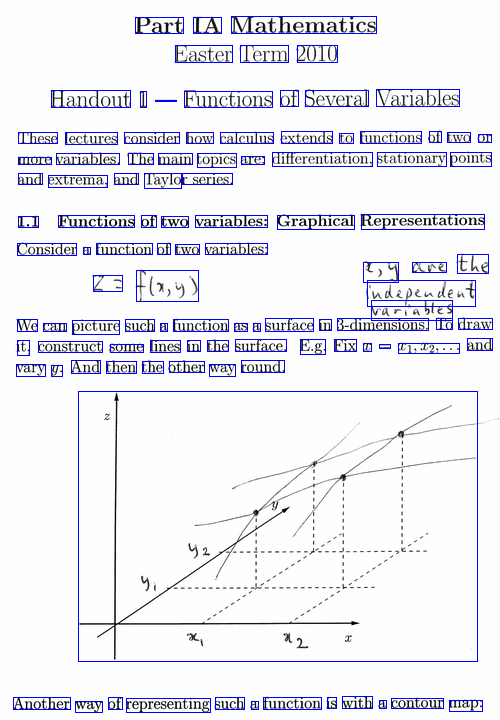
\includegraphics[width=\textwidth]{pla-word.png}
    \caption{Word scale}
  \end{subfigure}%
  \qquad
  \begin{subfigure}{.42\textwidth}
    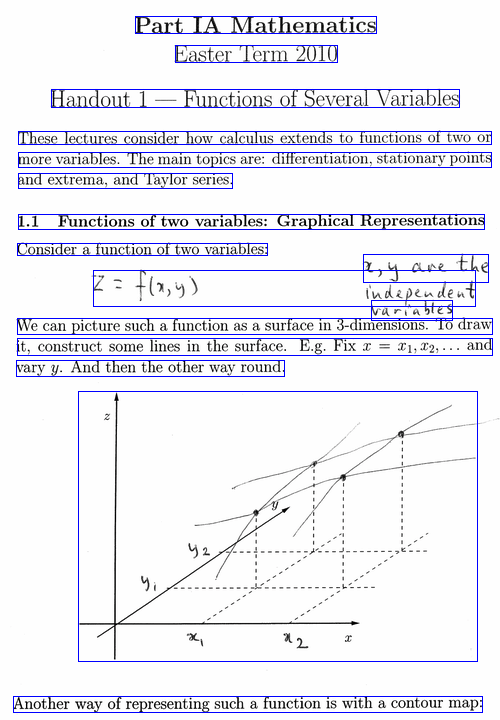
\includegraphics[width=\textwidth]{pla-line.png}
    \caption{Line scale}
  \end{subfigure}
  \vskip\baselineskip
  \begin{subfigure}{.42\textwidth}
    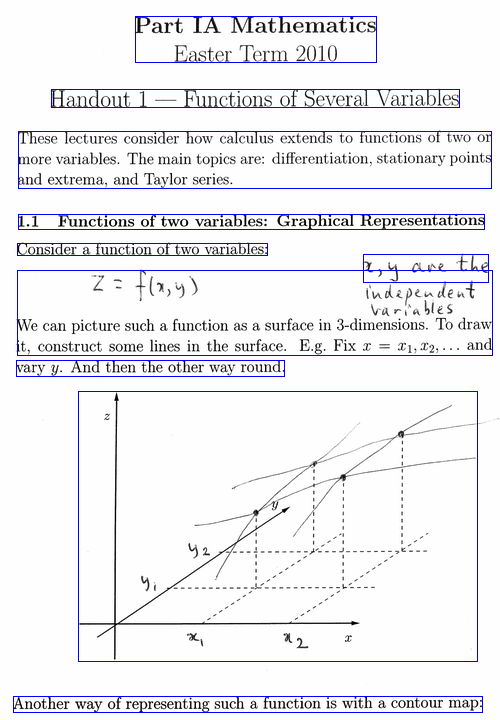
\includegraphics[width=\textwidth]{pla-par.png}
    \caption{Paragraph scale}
  \end{subfigure}%
  \qquad
  \begin{subfigure}{.42\textwidth}
    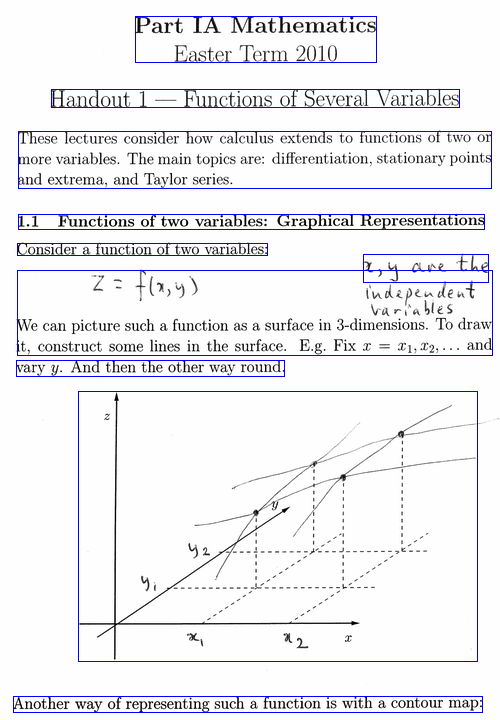
\includegraphics[width=\textwidth]{pla-block.png}
    \caption{Block scale}
  \end{subfigure}
  \caption{Different scales of Tesseract PLA}
  \label{fig:tess-pla-scales}
\end{figure}

In the actual system implementation, the user would be able to choose 4 different scales: word, line, paragraph and page. The `block' scale is removed from the implementation since in practice the difference between the `block' scale and the `paragraph' scale is negligible (which can be seen from \Cref{fig:tess-pla-scales}), and we keep the `paragraph' scale since the name `paragraph' is less ambiguous than `block'. 

We also keep the `page' scale in the system implementation for evaluation purposes described in later chapters, though this scale is not actually useful in practical use. The choice of PLA scale is considered to be one of the system hyperparameters.

\section{Model Switching}

Tesseract provides a large number of different models to support text recognition of different human languages. The default model is for recognising English text, which is named as \texttt{eng} in the Tesseract specification. 

Tesseract allows us to fine-tune existing models to produce improved models, or retrain from scratch to make completely new models. In this project, we have fine-tuned the default English model using additional handwritten data, and have included the fine-tuned model in the system implementation. The training of Tesseract OCR is further discussed in later chapters. 

Tesseract also allows us to specify what model to use before running the OCR engine. Using different models will eventually generate different recognition results. Therefore, the choice of the working Tesseract model is also one of the system hyperparameters.


